\documentclass[dvisvgm,tikz]{standalone}
\usepgflibrary{arrows.meta}
\renewcommand{\familydefault}{\sfdefault}

% latex pic.tex; dvisvgm --clipjoin --bbox=papersize --page=1- pic.dvi ; mv pic.svg filename.svg

\newcommand{\sllnode}[3]{
    \draw[black,thick,rotate=#3] (#1,#2) +(-10,0) rectangle +(10,10);
    \draw[rotate=#3] (#1,#2) +(0,5) node {\centering \rotatebox{#3}{Payload}};
    \draw[black,thick,rotate=#3] (#1,#2) +(-10,0) rectangle +(10,-10);
    \draw[rotate=#3] (#1,#2) +(0,-5) node {\centering \rotatebox{#3}{Next}};
}

\newcommand{\dllnode}[3]{
    \draw[black,thick,rotate=#3] (#1,#2) +(-10,0) rectangle +(10,10);
    \draw[rotate=#3] (#1,#2) +(0,5) node {\centering \rotatebox{#3}{Payload}};
    \draw[black,thick,rotate=#3] (#1,#2) +(0,0) rectangle +(10,-10);
    \draw[rotate=#3] (#1,#2) +(5,-5) node {\centering \rotatebox{#3}{Next}};
    \draw[black,thick,rotate=#3] (#1,#2) +(-10,0) rectangle +(0,-10);
    \draw[rotate=#3] (#1,#2) +(-5,-5) node {\centering \rotatebox{#3}{Prev}};
}

\begin{document}
    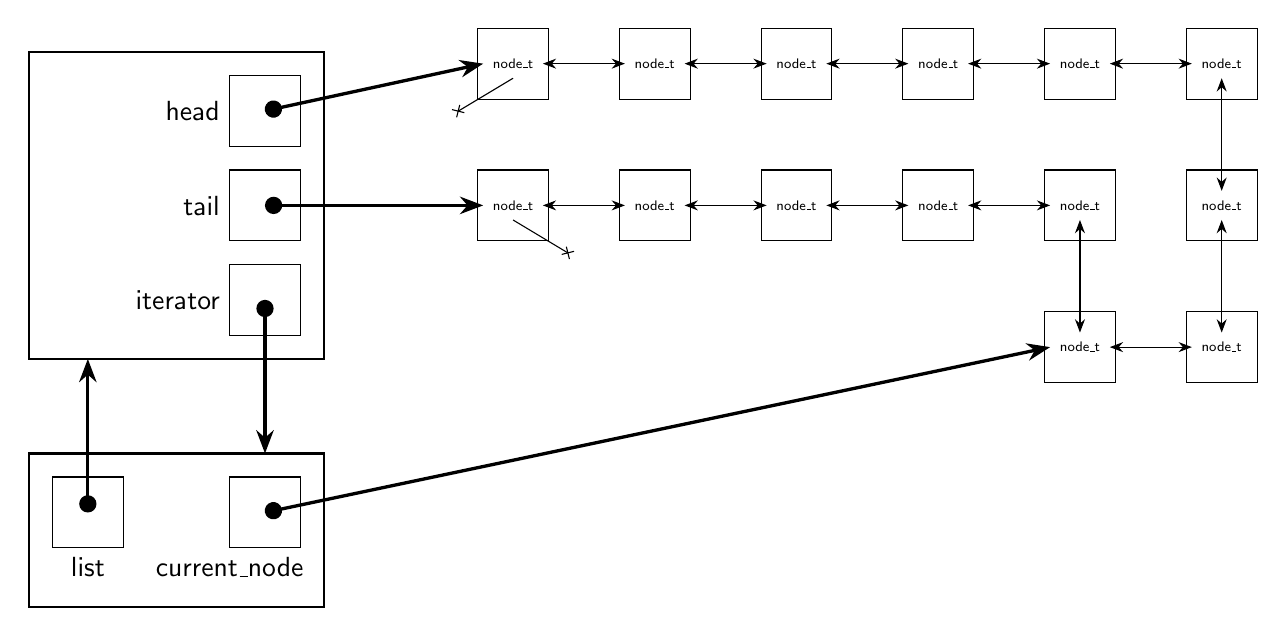
\begin{tikzpicture}[x=1.5mm, y=1.5mm]
        \draw[thick] (0,0) rectangle (25,26);
        \draw (17,24) rectangle ++(6,-6) +(-6,3) node[anchor=east] {head};
        \draw (17,16) rectangle ++(6,-6) +(-6,3) node[anchor=east] {tail};
        \draw (17,8)  rectangle ++(6,-6) +(-6,3) node[anchor=east] {iterator};
        \draw[Circle-Stealth,very thick] (20,5) -- (20,-8);

        \draw[thick] (0,-8) rectangle ++(25,-13);
        \draw (17,-10) rectangle ++(6,-6) +(-6,0) node[anchor=north] {current\_node};
        \draw (2,-10) rectangle ++(6,-6) +(-3,0) node[anchor=north] {list};
        \draw[Circle-Stealth,very thick] (5,-13) -- (5,0);

        \draw (38,28) rectangle ++(6,-6) +(-3,3) node (head) {\tiny{node\_t}};
        \draw[Circle-Stealth,very thick] (20,21) -- (head.west);
        \draw (38,16) rectangle ++(6,-6) +(-3,3) node (tail) {\tiny{node\_t}};
        \draw[Circle-Stealth,very thick] (20,13) -- (tail.west);
        \draw (86,4) rectangle ++(6,-6) +(-3,3) node (current) {\tiny{node\_t}};
        \draw[Circle-Stealth,very thick] (20,-13) -- (current.west);

        \draw (38,28)
        ++(12,0) rectangle ++(6,-6) ++(-3,3) node (node1) {\tiny{node\_t}}
        ++(9,3) rectangle ++(6,-6) ++(-3,3) node (node2) {\tiny{node\_t}}
        ++(9,3) rectangle ++(6,-6) ++(-3,3) node (node3) {\tiny{node\_t}}
        ++(9,3) rectangle ++(6,-6) ++(-3,3) node (node4) {\tiny{node\_t}}
        ++(9,3) rectangle ++(6,-6) ++(-3,3) node (node5) {\tiny{node\_t}}
        ++(-3,-9) rectangle ++(6,-6) ++(-3,3) node (node6) {\tiny{node\_t}}
        ++(-3,-9) rectangle ++(6,-6) ++(-3,3) node (node7) {\tiny{node\_t}}
        ++(-15,15) rectangle ++(6,-6) ++(-3,3) node (node8) {\tiny{node\_t}}
        ++(-15,3) rectangle ++(6,-6) ++(-3,3) node (node9) {\tiny{node\_t}}
        ++(-15,3) rectangle ++(6,-6) ++(-3,3) node (node10) {\tiny{node\_t}}
        ++(-15,3) rectangle ++(6,-6) ++(-3,3) node (node11) {\tiny{node\_t}};

        \draw[Stealth-Stealth] (head.east) -- (node1.west);
        \draw[Stealth-Stealth] (node1.east) -- (node2.west);
        \draw[Stealth-Stealth] (node2.east) -- (node3.west);
        \draw[Stealth-Stealth] (node3.east) -- (node4.west);
        \draw[Stealth-Stealth] (node4.east) -- (node5.west);
        \draw[Stealth-Stealth] (node5.south) -- (node6.north);
        \draw[Stealth-Stealth] (node6.south) -- (node7.north);
        \draw[Stealth-Stealth] (node7.west) -- (current.east);
        \draw[Stealth-Stealth] (current.north) -- (node8.south);
        \draw[Stealth-Stealth] (node8.west) -- (node9.east);
        \draw[Stealth-Stealth] (node9.west) -- (node10.east);
        \draw[Stealth-Stealth] (node10.west) -- (node11.east);
        \draw[Stealth-Stealth] (node11.west) -- (tail.east);

        \draw[-Rays] (head.south) -- ++(-5,-3);
        \draw[-Rays] (tail.south) -- ++(5,-3);
    \end{tikzpicture}
\end{document}